%%%%%=== background ===%%%%%
\chapter{系统需求与方案设计}
\thispagestyle{fancy}
根据本系统的应用需求,系统需要具备目标搜索、自主避障、移动降落等功能。

根据模块化设计原则,本系统的模块划分如图\ref{系统模块划分}所示:

\begin{figure}[h]
    \centering
    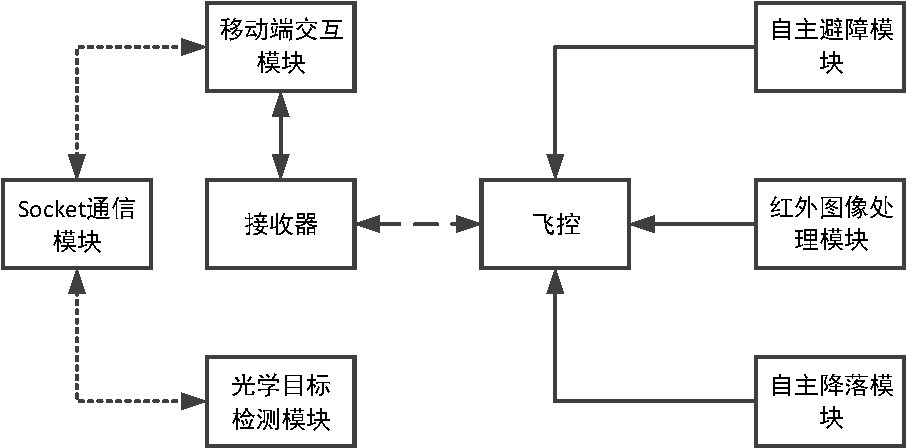
\includegraphics[width=14cm]{figures/系统模块划分.pdf}
    \caption{系统模块划分}\label{系统模块划分}
\end{figure}

由各个模块负责的功能以及数据输入输出接口,可以得到系统的工作数据链路图如图\ref{系统工作数据链路图}所示。

\begin{figure}[h]
    \centering
    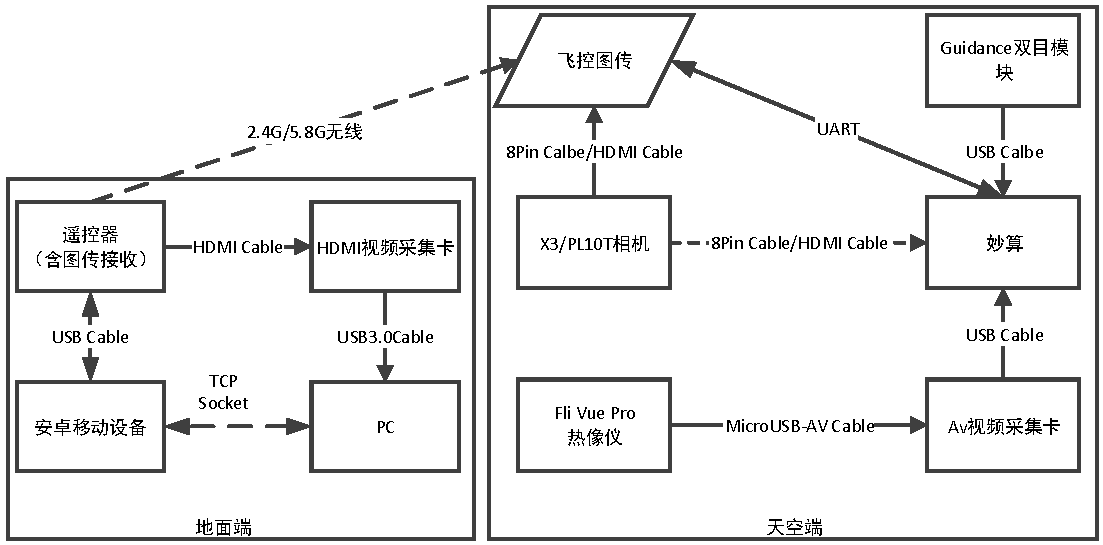
\includegraphics[width=14cm]{figures/系统工作数据链路图.pdf}
    \caption{系统工作数据链路图}\label{系统工作数据链路图}
\end{figure}

首先是无人机端。对于DJI M100无人机,云台相机的视频流通过8Pin电缆连接至无人机的高清图传的视频输入端。高清图传往地面站实时传送无人机视角画面。热成像仪FLIR VUE Pro的模拟视频接口通过USB-AV电缆传送至USB视频采集卡并连接至机载计算设备妙算Manifold进行处理。

Guidance避障模块的左右视图数据通过USB电缆连接至妙算Manifold进行分析处理。Manifold则通过UART串口连接线和DJI M100飞控进行通信。

地面端的数据接收主要依靠DJI M100配套的遥控器。值得注意的是,由于现在的无人机平台基本上都会配备高清图传模块,地面端的图传接收器通常和遥控器集成在一起,且通常都会有相应的视频输出接口以方便外接显示,如DJI M100的配套遥控器。如果使用自己组装的无人机平台,遥控器和图传接收分离开来,只需要从图传的视频输入端口采集视频数据。通过一个HDMI高清视频采集卡,地面端的笔记本电脑可以采集到实时回传的视频画面并进行处理。

遥控器和移动设备通过Mini-USB线缆连接。此外,移动设备和笔记本电脑将被设置到同一个网络,组建局域网,两者之间通过socket进行通信。
